% !TEX TS-program = pdflatex
% !TEX encoding = UTF-8 Unicode

% This is a simple template for a LaTeX document using the "article" class.
% See "book", "report", "letter" for other types of document.

\documentclass[11pt]{article} % use larger type; default would be 10pt

\usepackage[utf8]{inputenc} % set input encoding (not needed with XeLaTeX)
\usepackage{array}

\usepackage{float}

\usepackage{graphicx} % support the \includegraphics command and options
\usepackage[outdir=./]{epstopdf}
\usepackage{psfrag}

\usepackage{feynmp-auto}

\makeatletter
\def\endfmffile{%
  \fmfcmd{\p@rcent\space the end.^^J%
          end.^^J%
          endinput;}%
  \if@fmfio
    \immediate\closeout\@outfmf
  \fi
  \IfFileExists{\thefmffile.mp}{\immediate\write18{mpost \thefmffile}}{}
  \let\thefmffile\relax
}
\makeatother
%%% Examples of Article customizations
% These packages are optional, depending whether you want the features they provide.
% See the LaTeX Companion or other references for full information.

%%% PAGE DIMENSIONS
\usepackage{geometry} % to change the page dimensions
\geometry{a4paper} % or letterpaper (US) or a5paper or....
% \geometry{margin=2in} % for example, change the margins to 2 inches all round
% \geometry{landscape} % set up the page for landscape
%   read geometry.pdf for detailed page layout information

\usepackage{graphicx} % support the \includegraphics command and options

% \usepackage[parfill]{parskip} % Activate to begin paragraphs with an empty line rather than an indent

%%% PACKAGES
\usepackage{booktabs} % for much better looking tables
\usepackage{array} % for better arrays (eg matrices) in maths
\usepackage{paralist} % very flexible & customisable lists (eg. enumerate/itemize, etc.)
\usepackage{verbatim} % adds environment for commenting out blocks of text & for better verbatim
\usepackage{subfig} % make it possible to include more than one captioned figure/table in a single float
% These packages are all incorporated in the memoir class to one degree or another...

%%% HEADERS & FOOTERS
\usepackage{fancyhdr} % This should be set AFTER setting up the page geometry
\pagestyle{fancy} % options: empty , plain , fancy
\renewcommand{\headrulewidth}{0pt} % customise the layout...
\lhead{}\chead{}\rhead{}
\lfoot{}\cfoot{\thepage}\rfoot{}

%%% SECTION TITLE APPEARANCE
\usepackage{sectsty}
\allsectionsfont{\sffamily\mdseries\upshape} % (See the fntguide.pdf for font help)
% (This matches ConTeXt defaults)

%%% ToC (table of contents) APPEARANCE
\usepackage[nottoc,notlof,notlot]{tocbibind} % Put the bibliography in the ToC
\usepackage[titles,subfigure]{tocloft} % Alter the style of the Table of Contents
\renewcommand{\cftsecfont}{\rmfamily\mdseries\upshape}
\renewcommand{\cftsecpagefont}{\rmfamily\mdseries\upshape} % No bold!

%%% END Article customizations

%%% The "real" document content comes below...

\title{Rapport de stage - LAPP}
%\date{} % Activate to display a given date or no date (if empty),
         % otherwise the current date is printed 

% TODO : restructurer ce qui est écrit par avance

\begin{document}
\maketitle

\abstract{brouillon}

\section{Le LHC}

\section{Boson de Higgs}

\subsection{Caractéristiques}

Le boson de Higgs est une particule élémentaire du modèle standard de masse $\simeq$ 125 GeV et de spin nul et dont l'existence à été confortée par les résultats des expériences CMS et Atlas.

\subsection{Formation}

Il existe de nombreux processus entrainant la production de boson de Higgs. En voici des exemples envisageables ainsi que leur section efficace associée dans les conditions du LHC (Run1, $\sqrt{s} = $ 8 TeV).

\subsubsection{Fusion gluon gluon ($gg \to H$)}

La fusion gluon gluon est le mode de production du Higgs le plus important. 

La section efficace totale du processus est de 19,23 pb à $\sqrt{s} =$ 8 TeV et 43,94 pb à $\sqrt{s} =$ 13 TeV

\begin{fmffile}{gg_H}
\begin{figure}[H]
      \centering
\begin{fmfgraph*}(175,125)
\fmfleft{i1,i2}
\fmfright{o1}

\fmflabel{$g$}{i1}
\fmflabel{$g$}{i2}
\fmflabel{$H$}{o1}

\fmf{gluon}{i1,v1}
\fmf{gluon}{i2,v2}
\fmf{dashes}{v3,o1}
\fmf{fermion,label=$q$}{v1,v2}
\fmf{fermion}{v2,v3}
\fmf{fermion}{v3,v1}
\end{fmfgraph*}
\caption{Formation d'un Higgs par fusion de gluons (avec apparition de quarks virtuels, préférentiellement lourds).  }
\end{figure}
\end{fmffile}

\subsubsection{Vector Boson Fusion (VBF, $ff \to ffH$)}

La section efficace du processus VBF est de 1,58 pb à $\sqrt{s} =$ 8 TeV et 3,75 à $\sqrt{s} =$ 13 TeV. Il s'agit du second mode de production du Higgs le plus probable.

\begin{fmffile}{VBF}
\begin{figure}[H]
      \centering
\begin{fmfgraph*}(175,125)
\fmfleft{i1,i2}
\fmfright{o1,o2,o3}

\fmflabel{$f$}{i1}
\fmflabel{$f$}{i2}
\fmflabel{$f$}{o1}
\fmflabel{$f$}{o3}
\fmflabel{$H$}{o2}
\fmflabel{$W,Z$}{v3}

\fmf{fermion}{i1,v1,o1}
\fmf{fermion}{i2,v2,o3}
\fmf{photon}{v1,v3}
\fmf{photon}{v3,v2}
\fmf{dashes}{v3,o2}
\end{fmfgraph*}
\caption{Formation d'un Higgs par fusion de bosons $W$ ou $Z$ virtuels échangés entre deux fermions.  }
\end{figure}
\end{fmffile}

\subsubsection{Higgs Strahlung ($f\bar{f} \to WH \textrm{ ou } ZH$)}

La section efficace totale pour ce processus est $\sigma = \sigma_W + \sigma_Z$ = 0,7 $+$0,4 = 1,1 pb à $\sqrt{s} =$ 8 TeV et $\sigma =$ 2,3 à $\sqrt{s}$ = 13 TeV

\begin{fmffile}{HS}
\begin{figure}[H]
      \centering
\begin{fmfgraph*}(175,125)
\fmfleft{i1,i2}
\fmfright{o1,o2}

\fmflabel{$f$}{i1}
\fmflabel{$\bar{f}$}{i2}
\fmflabel{$W,Z$}{o1}
\fmflabel{$H$}{o2}

\fmf{fermion}{i1,v1}
\fmf{fermion}{v1,i2}
\fmf{photon,label=$W,,Z$}{v1,v2}
\fmf{photon}{v2,o1}
\fmf{dashes}{v2,o2}
\end{fmfgraph*}
\caption{La collision d'un fermion avec un antifermion peut produire un boson $W$ ou $Z$ pouvant émettre un $H$. }
\end{figure}
\end{fmffile}

\subsubsection{Top/bottom fusion (ex: $gg \to q\bar{q}H$, $q = t,b$)}

\begin{fmffile}{TF}
\begin{figure}[H]
      \centering
\begin{fmfgraph*}(175,125)
\fmfleft{i1,i2}
\fmfright{o1,o2,o3}

\fmflabel{$g$}{i1}
\fmflabel{$g$}{i2}
\fmflabel{$q$}{o1}
\fmflabel{$H$}{o2}
\fmflabel{$\bar{q}$}{o3}

\fmf{gluon}{i1,v1}
\fmf{gluon}{i2,v2}

\fmf{fermion}{v1,o1}
\fmf{fermion}{o3,v2}
\fmf{fermion,label=$q$}{v2,v3}
\fmf{fermion,label=$\bar{q}$}{v3,v1}

\fmf{dashes}{v3,o2}
\end{fmfgraph*}
\caption{Ici, deux gluons produisent deux paires $t\bar{t}$ ou $b\bar{b}$. Une d'entre elles fusionne et produit un $H$. Il s'agit d'un processus mineur ($\sigma = \sigma_b + \sigma_t = $ 0,20 $+$ 0,13 = 0,33 pb)}
\end{figure}
\end{fmffile}

\begin{fmffile}{TF_2}
\begin{figure}[H]
      \centering
\begin{fmfgraph*}(175,125)
\fmfleft{i1,i2}
\fmfright{o1,o2,o3,o4}

\fmflabel{$q$}{i1}
\fmflabel{$\bar{q}$}{i2}
\fmflabel{$\over{b}$}{o1}
\fmflabel{$H$}{o2}
\fmflabel{$b$}{o3}

\fmf{fermion}{i1,v1}
\fmf{fermion}{v1,i2}
\fmf{gluon}{v1,v2}

\fmf{fermion}{v2,o3}

\fmf{fermion}{o1,v3}
\fmf{fermion}{v3,v2}
\fmf{dashes}{v3,o2}
\end{fmfgraph*}
\caption{Un autre exemple de production $q\bar{q}H$ (ici $q\bar{q} \to b\bar{b}H$)}
\end{figure}
\end{fmffile}

\subsection{Désintégration}

La liste suivante n'est pas exhaustive. Elle regroupe certains modes privilégiés (ratio de branche élevé, ou intérêt expérimental).

\begin{tabular}{|l|c|r|} 
   \hline
   Type & Exemple & Ratio de branche\\
    \hline
    H $\to$ fermions & $H \to b\bar{b} $ & 57,7 \% \\
    \cline{2-3} 
        & $H \to \tau\bar{\tau} $ & 6,4 \% \\
   \cline{2-3} 
        & $H \to \mu\bar{\mu}$ & 0,02 \%\\
    \hline
  H $\to$ bosons de jauge & $H \to WW$ &21,5 \% \\
   \cline{2-3}
      & $H \to \gamma \gamma$ & 0,23 \% \\
  \hline
\end{tabular}

% différentes voies, par importance et BR
% expliquer contraintes de détections et pq H->yy privilégié malgré faible BR etc..


\section{Atlas}

\subsection{Objectifs de l'expérience}

% à relier a ce qui a été dit précédemment sur H
\subsection{Détecteurs}
% inclure schémas

\subsection{Performance}
% efficacité (à relier aux schémas)
\subsection{}

\section{Données}

\subsection{Calcul de la masse du Higgs}

En connaissant l'énergie des photons produits de la désintégration du Higgs selon la forme $H\to \gamma \gamma$, on peut retrouver sa masse. Elle est en effet égale à la masse invariante du système 

\begin{equation}
m_{\textrm{inv}}^2 = E^2 - \textbf{p}^2
\end{equation}

Pour deux photons, $E_{\gamma_1} = p_{\gamma_1}$ et $E_{\gamma_2} = p_{\gamma_2}$, et alors :

\begin{equation}
m_{\gamma \gamma}^2 = 2 \left ( p_{\gamma_1} p_{\gamma_2} - \textbf{p}_{\gamma_1} . \textbf{p}_{\gamma_2} \right )
\end{equation}

Soit, en travaillant en coordonnées $(\eta, \phi)$ :

\begin{equation}
m_{\gamma \gamma}^2 = 2 E_{\gamma_1} E_{\gamma_2} \left [ \cosh {\left( \eta_{\gamma_1} - \eta_{\gamma_1} \right)} - \cos{\left( \phi_{\gamma_1} - \phi_{\gamma_1} \right)} \right ]
\end{equation}

Il s'agit alors de calculer cette masse pour tous les évènements contenant une paire de photons susceptible d'être issue d'un Higgs. Et 

\subsection{Calcul}

Parmi un échantillon de 310 000 évènements (constitués uniquement de paires de photons vérifiant le critère 'tight'), on calcule la distribution de masse invariante $m_{\gamma \gamma}$. On obtient le résultat suivant :

\begin{figure}[H]
\centering
  \caption{Distribution m$_{\gamma \gamma}$. On observe un bruit important avec un pic aux alentours de 90 GeV. Le signal correspondait au Higgs est à première vue difficilement distinguable. }
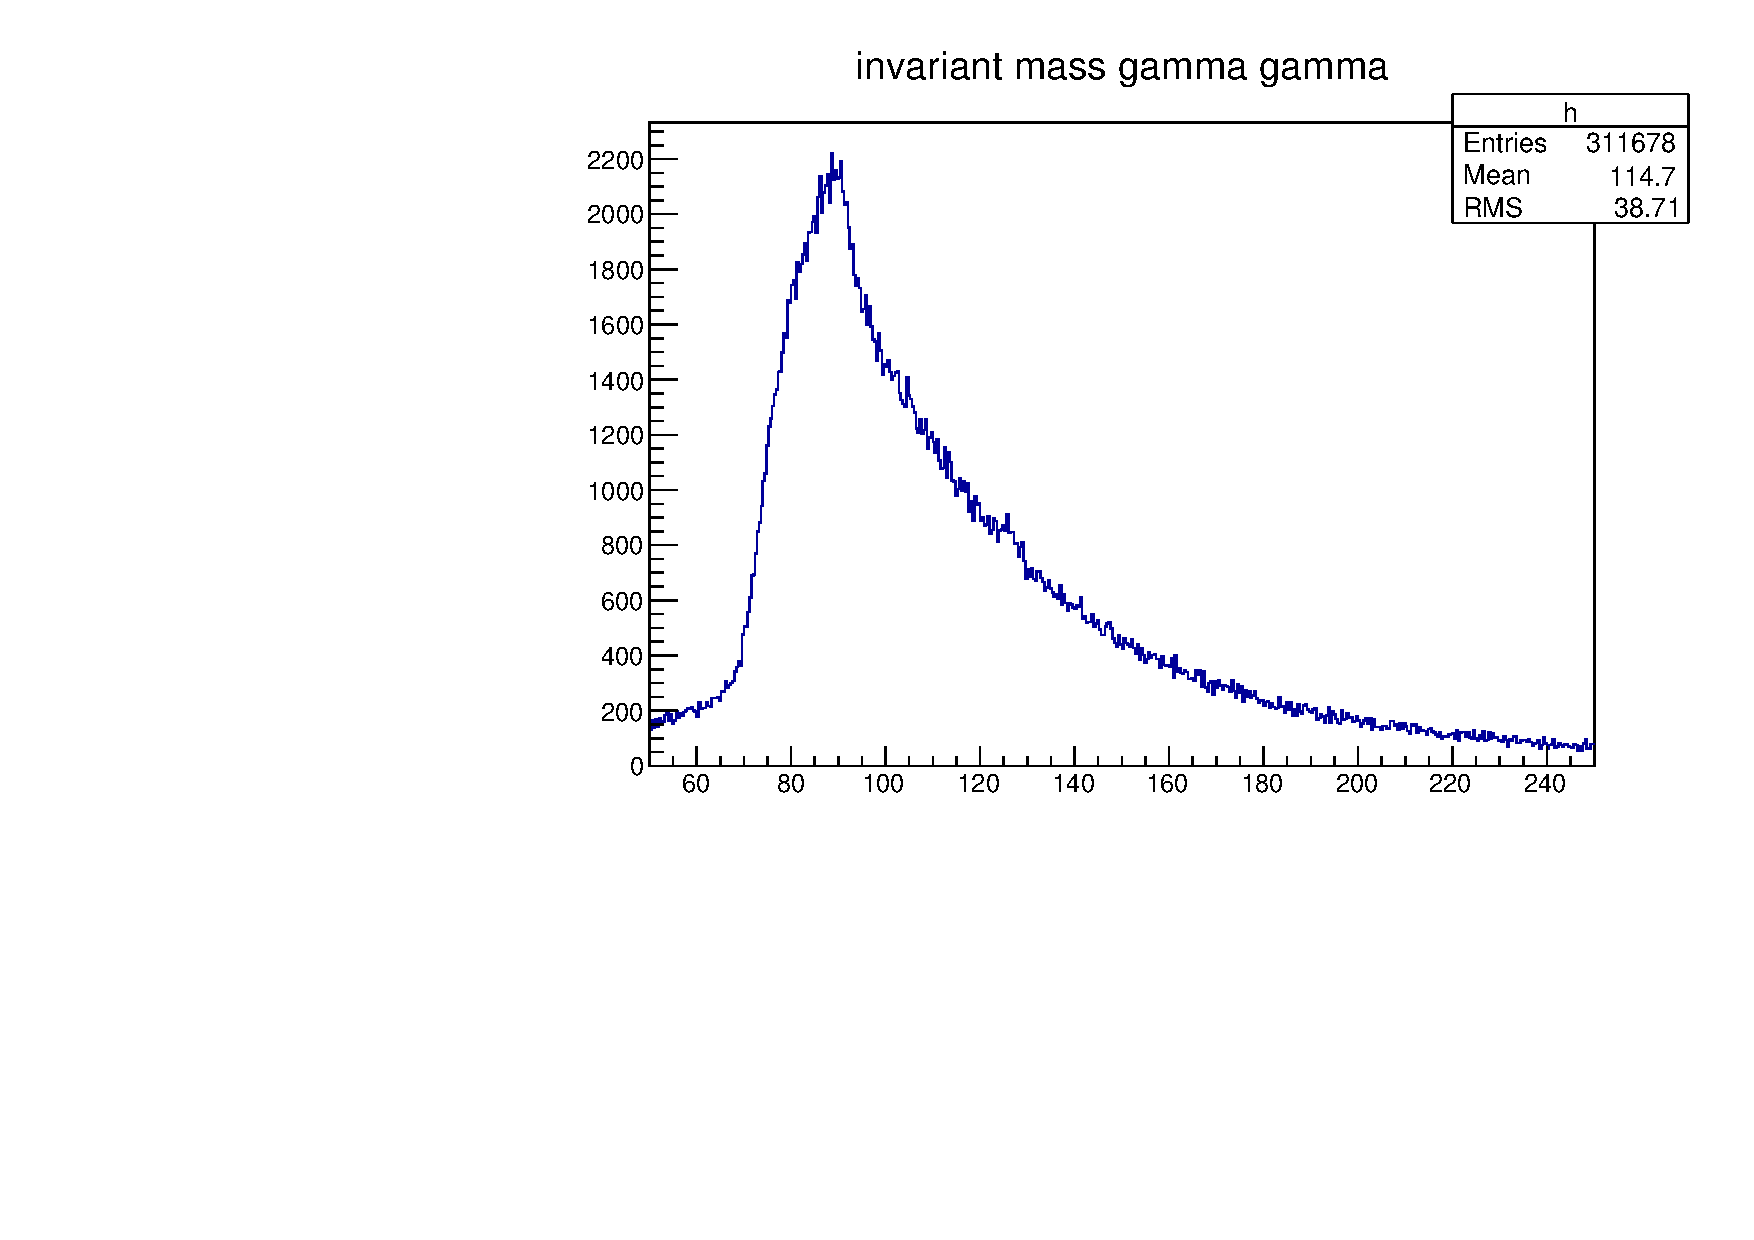
\includegraphics[width=500pt]{../graphes/mgg_medium}
\end{figure}

%Afin d'extraire le signal correspondant au Higgs, on se restreint à la plage où il est attendu (110 - 140 GeV). Le 'background' y suit une forme exponentielle. On en réalise alors un fit sur une zone ou le signal est considéré nul : ici on a choisi [110;120] $\cup$  [130;140]. On obtient une fonction de la forme $\textrm{background} = E \mapsto \exp(\xi + \epsilon E)$.
%
%Puis, sur la plage complète ([110, 140]), on réalise un fit des données à partir d'une fonction de la forme signal+background : $E \mapsto  A \exp\left(-(E-E_0)^2/2\sigma^2\right) + \exp(\xi + \epsilon E)$
%
%On obtient la figure suivante :
%
%\begin{figure}[H]
%  \caption{Distribution $m_{\gamma \gamma}$ et fit background+signal. }
%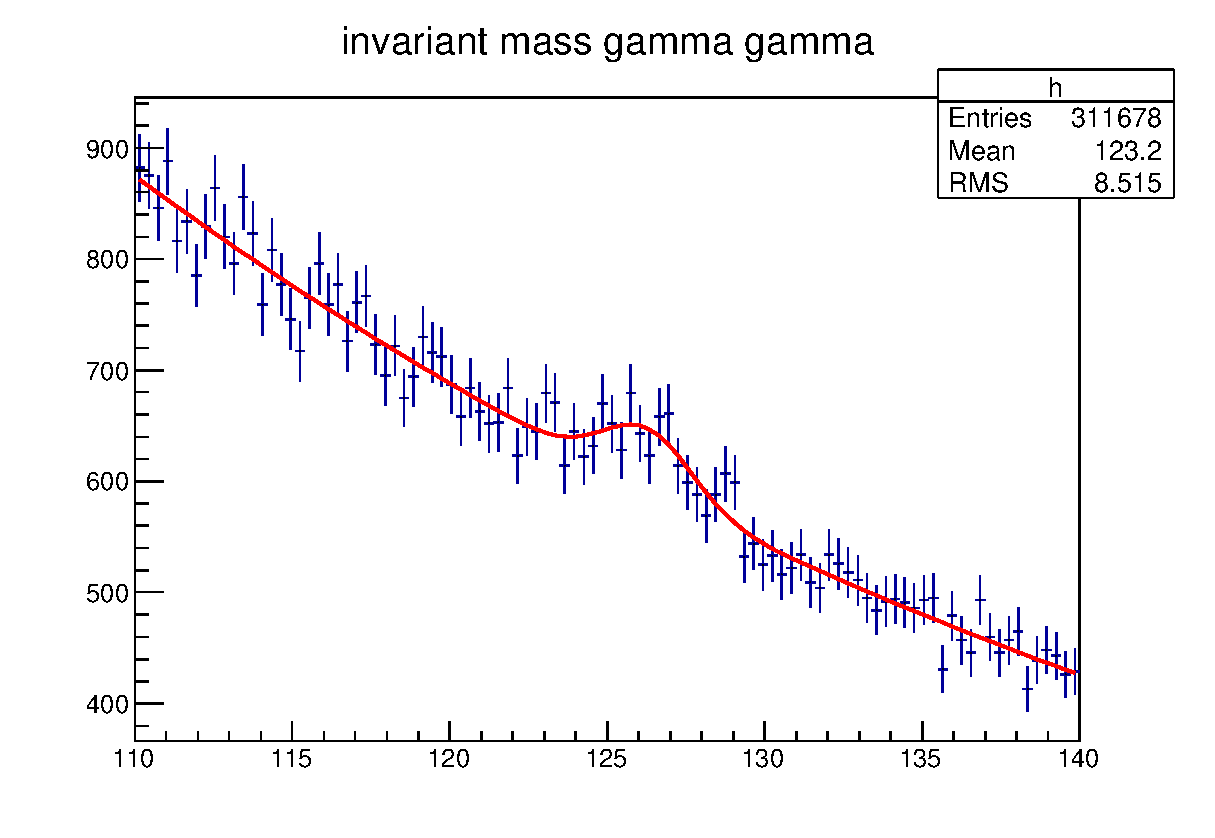
\includegraphics{../graphes/mgg_30GeV}
%\end{figure}
%
%On peut en déduire les paramètres physiquement intéressants suivants :
%
%\begin{tabular}{|l|c|r|} 
%   \hline
%   Paramètre & Valeur & Erreur \\
%    \hline
%   $E_0$ & 126,3 GeV & 0,3 GeV\\
%  \hline
%   $\sigma$ & 2,0 GeV & 0,9 GeV \\
%  \hline
%\end{tabular}
%
%La valeur $E_0$ doit correspondre à la masse du Higgs. On remarque qu'elle en est en effet bien proche (126 au lieu de 125 GeV). La valeur $\sigma$ doit correspondre à la largeur du signal, dont la valeur théorique attendue n'est pas nulle.
%
%On calcule de plus $\chi^2 = $ 68,8 pour un nombre de degrés de liberté égal à 99, ce qui correspond à une p-value de 99,0 \% (2,5$\sigma$?)
%$\Delta \chi^2 = \chi^2_{\textrm{background}} - \chi^2{\textrm{signal+background} \simeq 120-70 \simeq 50$ soit une significance à $\sqrt{\Delta \chi^2} \sigma = 7 \sigma$

Afin d'extraire le signal correspondant au Higgs, on se restreint à la plage où il est attendu (100 - 150 GeV). Le 'background' y suit une forme exponentielle. On en réalise alors un fit sur une zone ou le signal est considéré nul : ici on a choisi [100;120] $\cup$  [130;150]. On obtient une fonction de la forme $\textrm{background} = E \mapsto \exp(\xi + \epsilon E)$.

Puis, sur la plage complète ([100, 150]), on réalise un fit des données à partir d'une fonction de la forme signal+background : $E \mapsto  A \exp\left(-(E-E_0)^2/2\sigma^2\right) + \exp(\xi + \epsilon E)$

On obtient la figure suivante :

\begin{figure}[H]
\centering
  \caption{Distribution $m_{\gamma \gamma}$ et fit background+signal. }
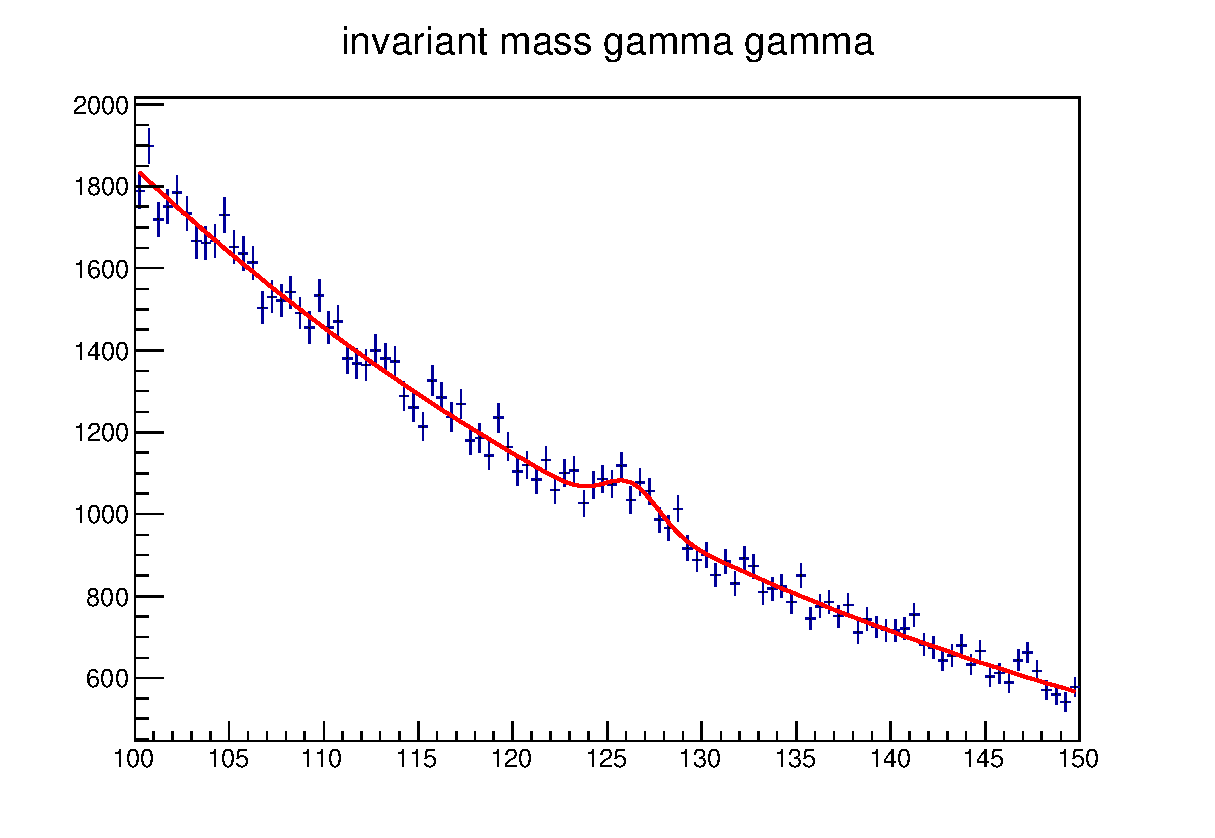
\includegraphics[width=500pt]{../graphes/mgg_50GeV}
\end{figure}

On peut en déduire les paramètres physiquement intéressants suivants :

\begin{tabular}{|l|c|r|} 
   \hline
   Paramètre & Valeur & Erreur \\
    \hline
   $E_0$ & 126,3 GeV & 0,3 GeV\\
  \hline
   $\sigma$ & 2,0 GeV & 0,9 GeV \\
  \hline
\end{tabular}

La valeur $E_0$ doit correspondre à la masse du Higgs. On remarque qu'elle en est en effet bien proche (126 au lieu de 125 GeV). La valeur $\sigma$ doit correspondre à la largeur du signal, dont la valeur théorique attendue n'est pas nulle.

On calcule d'autre part la significance statistique d'après ces fits : $\Delta \chi^2 = \chi^2_{\textrm{background}} - \chi^2_{\textrm{signal+background}} \simeq 155-107 \simeq 50$ soit une significance à $\sqrt{\Delta \chi^2} \ \sigma = 7 \sigma$


\end{document}
